\section{Correlação entre Depressão e estresse oxidativo}

Em pacientes deprimidos, constata-se um aumento transitório na secreção de cortisol, como ocorre no estresse agudo, suprimindo o sistema imunitário e atrasando o processo anti-inflamatório. \cite{Kandel} Em geral, grande parte dos antidepressivos comercializados atuam sobre as monoaminas. Entre as áreas mais promissoras na pesquisa de antidepressivos, está os que possam agir no eixo hipotálamo-adrenal. Isto porque, especula-se que os sintomas de um episódio depressivo possa ser atribuído aos níveis elevados de cortisol. \cite{Schatzberg2015}

\subsection{Polimorfismos nos genes 5-HTTLPR e FKBP5}

  No decorrer da vida, eventos estressantes que envolvem ameaças, perdas ou humilhação, influenciam o início e o curso da depressão. No entanto, nem todas as pessoas que enfrentam situações difíceis decaem num episódio depressivo. Verificou-se que um polimorfismo funcional na região promotora do gene transportador de serotonina (5-HTTLPR) modera, em partes, a resiliência perante eventos estressantes ao longo da vida. Indivíduos com uma ou duas cópias do alelo curto do polimorfismo exibiram mais sintomas depressivos, depressão diagnosticável e suicídio em relação a indivíduos homozigotos para o alelo longo. \cite{Caspi2003}
  
  O impacto das alterações epigenéticas em FKBP5 estão em parte relacionadas à resistência e descontrole hormonal de glicocorticóides, reduzindo as respostas inflamatórias refletidas pela diminuição da sensibilidade
  ao glicocorticóide sintético dexametasona in vitro. \cite{Klengel2013}
  
\section{Processos inflamatórios e a Depressão}

O impacto do sistema inflamatório na ocorrência de depressão foi reconhecido pela primeira vez em meados de 1990. \cite{Yang2012} Quantidades crescentes de estudos sugerem que as respostas inflamatórias têm um papel importante na fisiopatologia da depressão. Verificou-se que os pacientes deprimidos apresentam níveis mais altos de citocinas pró-inflamatórias, proteínas de fase aguda, quimiocinas e moléculas de adesão celular. \cite{Raison2006} Esses achados sugerem que o direcionamento de citocinas pró-inflamatórias e suas vias de sinalização podem representar uma nova estratégia para o tratamento da depressão.

Quando comparados com indivíduos saudáveis, os pacientes clinicamente doentes com depressão maior exibem todas as características principais de processos inflamatórios, incluindo elevações nas citocinas inflamatórias relevantes e seus receptores solúveis no sangue periférico. \cite{Raison2009}

Também foram descritas associações entre sinais inflamatórios e sintomas depressivos individuais, como fadiga, atraso cognitivo e distúrbios do sono. Além do mais, processos inflamatórios também caracterizam-se por alterações no metabolismo de neurotransmissores, função neuroendócrina e plasticidade neural.\cite{Raison2009} 

Um grande estudo realizado em 2010 relata concentrações significativamente mais altas das citocinas pró-inflamatórias TNF-$\alpha$ e IL-6 em indivíduos deprimidos em comparação com o grupo controle. Embora resultados positivos e negativos venham sido relatados na literatura, esse resultado meta-analítico reforça as evidências de que a depressão é acompanhada pela ativação do sistema IRS. \cite{Dawlati2010}

Os níveis de duas citocinas, interleucina-6 (IL-6) e fator de necrose tumoral-$\alpha$ (TNF-$\alpha$) aumentaram de forma significativa em pacientes com estado grave de transtornos bipolares, depressivos e esquizofrenia em comparação com grupo controle. \cite{Miller2016}

As citocinas inflamatórias são nitidamente mais elevadas na depressão aguda e podem estar associadas à resistência ao tratamento monoaminérgico. Meta-análises confirmam níveis elevados de citocinas inflamatórias circulantes em pacientes deprimidos, e estudos longitudinais demonstraram que níveis elevados de citocinas séricas precedem sintomas depressivos. \cite{Kappelmann2018}

\begin{figure}[H]
\centering
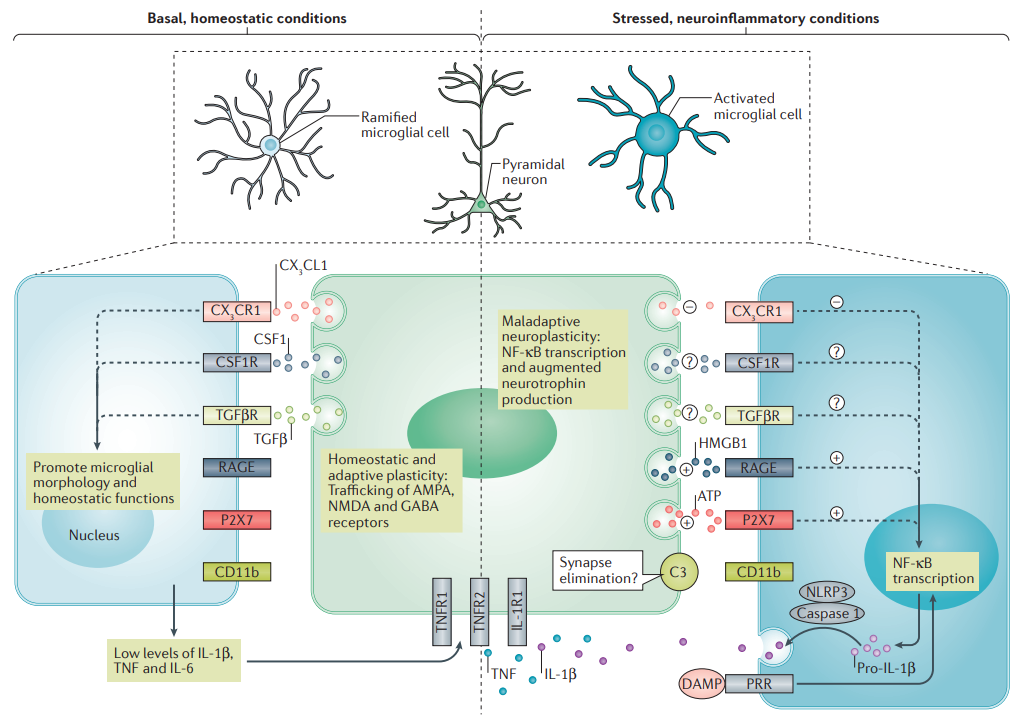
\includegraphics[scale=1]{Figuras/immunitary_system.png}
\caption{Interações bioquímicas entre microglia-neurônio num cérebro saudável e condições homeostáticas, em comparação a um cérebro sob condições de estresse ou deprimido. \cite{Iwata2016}}
\end{figure}

\begin{table}[H]
\caption {Proteínas envolvidas em processos inflamatórios que podem ser de grande ajuda na busca de novos fármacos para o tratamento da depressão.\cite{Raison2009} (Adaptado)} 
    \begin{tcolorbox}[tab1,tabularx={XYYY},title= Alvos promissores do sistema inflamatório,boxrule=0.5pt]
    
    \centering{\textbf{Immune System} & \textbf{Central Nervous System}     &  \textbf{Neuroendocrine System}     &  \textbf{Autonomic Nervous System}}  \\ \hline \\
    
    \centering{Cytokines: \textit{TNF-alpha, IL-1, IL-6}   & Monoamines: \textit{5-HT, NE, DA} & HPA axis hormones: \textit{CRH, cortisol} & Catecholamines: \textit{alpha and beta adrenergic}}\\ \\
    
    \centering{Cytokine signalling: \textit{$NF-\kappa B$, MAPK} & IDO and its metabolites: \textit{KYN, QUIN, KA}  & HPA receptors: \textit{GR} & Parasympathetic outflow pathways: \textit{vagal nerve, alpha 7 and nAChR} }  \\
    
    \centering{Inflammatory mediators: \textit{COX-2, PG} & Extrasynaptic NMDA receptors}   \\ \\
    
    \centering{Reactive nitrogen/oxygen species: \textit{NO, $H_2O_2$}  &  Excitotoxic neurotransmitters: \textit{glutamate} & &} \\ \\
    
    \centering{Immune cells in the brain: \textit{microglia} & Neurotrophic factors: \textit{BDNF}}
    
    \end{tcolorbox}
\end{table}

A ativação de células T efetoras durante o estresse pode impedir o desenvolvimento de comportamentos depressivos e de ansiedade. Esses efeitos produzem células de resposta anti-inflamatória IL-4, que estimulam a produção de fatores de crescimento no cérebro que apoiam a neuroplasticidade e resiliência. \cite{Evolution2016} 

Vem sendo consolidado a visão de que processos imunológicos podem estar significativamente envolvidos na resposta ao tratamento em transtornos afetivos. \cite{Lanquillon2000}